% !TeX root = ../../Book1.tex
% 纲要标题：### 2.5 圆锥曲线上的构造与定理
% 纲要位置：几何学计划纲要.md，第 185 行。
% 正文状态：初稿；尚未正式审核。

% 纲要内容开始
% 
% * 由投影得到有理参数及其逆
% * 圆锥曲线上的交比
% * Pascal 定理的坐标证明
% * Brianchon 定理与对偶推导
% 
% 纲要内容结束

\section{圆锥曲线上的构造与定理}
\label{g1:sec:0205}

射影分类告诉我们哪些圆锥曲线可以通过换坐标互相变换，但还没有说明怎样在一条曲线上移动和构造点。一个可操作的办法是固定曲线上一点，让过它的直线转动，用直线与曲线的另一个交点作参数。这样，圆锥曲线上的计算转化为射影直线上的计算；交比因此有了新的适用对象，而六个点的关联关系也能压缩为含三个参数的多项式恒等式。

\subsection{由投影得到有理参数及其逆}
\label{g1:subsec:0205:01}

本节讨论 \(K=\mathbb R\) 或 \(\mathbb C\) 上的非退化圆锥曲线，即射影平面中由可逆对称矩阵给出的二次方程。实数域上还须要求存在实点；例如 \(X^2+Y^2+Z^2=0\) 没有实射影点，不能从 \(\mathbb P^1(\mathbb R)\) 参数化一个空集。由\cref{g1:thm:projective-quadric-classification}，复数域上的非退化三元型都等价于 \(X^2+Y^2+Z^2\)，它含有点 \([1:\mathrm i:0]\)，所以在复数域上非空条件自动满足。下面仍把一个曲线点作为构造的输入，从它直接找出参数坐标。

\begin{proposition}[圆锥曲线的参数化]\label{g1:prop:conic-parametrization}
	设 \(K=\mathbb R\) 或 \(\mathbb C\)，\(C\subseteq\mathbb P^2(K)\) 是非退化圆锥曲线，且有一个 \(K\)-点。则存在射影坐标使 \(C\) 的方程为 \(XZ-Y^2=0\)。在这些坐标中，映射
	\begin{equation}\label{g1:eq:conic-parametrization}
		\nu:\mathbb P^1(K)\longrightarrow C,
		\qquad [s:t]\longmapsto[s^2:st:t^2]
	\end{equation}
	是双射。逆映射在 \(Z\ne0\) 上为 \([X:Y:Z]\mapsto[Y:Z]\)，在 \(X\ne0\) 上为 \([X:Y:Z]\mapsto[X:Y]\)，二者在交集上一致。
\end{proposition}
\begin{proof}
	先说明坐标为何存在。写 \(q(v)=B(v,v)\)，取非零 \(v\) 满足 \(q(v)=0\)。非退化性使我们能选 \(w\) 满足 \(B(v,w)=1\)。令 \(w'=w-\frac12q(w)v\)，则 \(q(w')=0\)、\(B(v,w')=1\)。在 \(H=\operatorname{span}(v,w')\) 上，配对矩阵为 \(\left(\begin{smallmatrix}0&1\\1&0\end{smallmatrix}\right)\)，可逆。因此每个向量可唯一减去 \(v,w'\) 的线性组合而变成与 \(H\) 正交的向量：两个待定系数由这一个可逆矩阵确定。于是 \(V=H\oplus H^{\perp_B}\)，且后一空间为一维。取其非零生成元 \(u\)，必有 \(a=q(u)\ne0\)，否则 \(u\) 与整个 \(V\) 正交，违反非退化性。故
	\[
		q(\alpha v+\beta w'+\gamma u)=2\alpha\beta+a\gamma^2.
	\]
	置 \(\alpha=X\)、\(\beta=-aZ/2\)、\(\gamma=Y\)，零点方程就变成 \(XZ-Y^2=0\)。

	接着核对参数映射。\(s,t\) 不全为零时三个二次单项式不全为零，把 \((s,t)\) 乘 \(\lambda\ne0\) 只将像乘 \(\lambda^2\)，故良定义，且像满足曲线方程。若 \(Z\ne0\)，方程给出
	\[
		[X:Y:Z]=[(Y/Z)^2:Y/Z:1]=\nu([Y:Z]).
	\]
	若 \(Z=0\)，必有 \(Y=0\)，该点为 \([1:0:0]=\nu([1:0])\)。在 \(X\ne0\) 的图上同样得到逆公式 \([X:Y]\)。两图覆盖 \(C\)，因为 \(X=Z=0\) 会迫使所有坐标为零；交集上 \([X:Y]=[Y:Z]\) 正是 \(XZ=Y^2\)。这证明满射和逆映射的唯一性。
\end{proof}

在 \(t\ne0\) 的参数图上置 \(r=s/t\)，便有 \(\nu(r)=[r^2:r:1]\)；缺少的一个点记作 \(\nu(\infty)=[1:0:0]\)。这种用参数的有理函数表示坐标的方式称为\term[youlicanshuhua]{有理参数化}[rational parametrization]。两个参数图各自有公式，在交集相容，共同覆盖整条曲线。

\begin{figure}[htbp]
	\centering
	% !TeX root = ../Book1.tex
\begin{tikzpicture}[scale=1.5]
	\draw[->,gray] (-1.5,0)--(1.6,0) node[right]{\(x\)};
	\draw[->,gray] (0,-1.25)--(0,1.35) node[above]{\(y\)};
	\draw[thick] (0,0) circle (1);
	\draw[blue!65!black] (-1.4,-0.2)--(1.4,1.2);
	\draw[gray,dashed] (-1,-1.2)--(-1,1.25);
	\draw[gray,dotted] (0.6,0)--(0.6,0.8)--(0,0.8);
	\fill (-1,0) circle (1.1pt) node[below left]{\(P=(-1,0)\)};
	\fill (0.6,0.8) circle (1.1pt) node[above left]{\(Q(m)\)};
	\node[blue!65!black,right] at (1.12,0.96) {\(y=m(x+1)\)};
	\node[left] at (-1,1.13) {切线};
	\node[below right] at (0,0) {\(0\)};
\end{tikzpicture}

	\caption[圆上的投影参数]{圆上的投影参数。固定 \(P=(-1,0)\)，过 \(P\) 的直线由斜率 \(m\) 标记；第二交点给出圆的参数化。切线 \(x=-1\) 对应参数直线上的无穷远点，并在延拓后对应 \(P\) 本身。}
	\label{g1:fig:conic-projection}
\end{figure}

这个双射正来自投影。对标准曲线固定 \(O=\nu(\infty)\)，过 \(O\) 的直线写成 \(tY-sZ=0\)，由 \([s:t]\in\mathbb P^1(K)\) 参数化。若 \(t\ne0\)，该直线与曲线相交于 \(O\) 和 \(\nu([s:t])\)；若 \(t=0\)，它成为 \(Z=0\)，即 \(O\) 处的切线。所以“另一个交点”的构造原先漏掉了 \(O\)，补上切线所对应的参数后，才得到整条曲线上的双射。

\begin{example}[单位圆的有理公式]\label{g1:exm:circle-parametrization}
	在实平面取 \(P=(-1,0)\)，直线 \(y=m(x+1)\) 与 \(x^2+y^2=1\) 相交。代入得到 \((x+1)((1+m^2)x+m^2-1)=0\)。把已知根 \(x=-1\) 提出后，另一个根为
	\[
		x=\frac{1-m^2}{1+m^2},\qquad y=\frac{2m}{1+m^2}.
	\]
	反过来，圆上除 \(P\) 外的点满足 \(m=y/(x+1)\)。参数 \(m=\infty\) 对应竖直切线，并补回点 \(P\)，如\cref{g1:fig:conic-projection}所示。这比三角函数参数更适合只涉及直线求交和代数计算的问题；两种参数表达同一个圆，却保留不同的计算便利。
\end{example}

\subsection{圆锥曲线上的交比}
\label{g1:subsec:0205:02}

先观察一条曲线上的四个点怎样变成射影直线上的四个点。过固定点 \(P\) 的全部直线称为以 \(P\) 为中心的\term[xianshu]{线束}[pencil of lines]。若 \(P=[p]\)，这些直线系数构成二维子空间 \((Kp)^\circ\) 的射影化，所以线束本身就是一条射影直线。这说明可以对四条线定义交比，但还须证明结果与投影中心无关。

\begin{proposition}[曲线交比的选择无关性]\label{g1:prop:conic-cross-ratio}
	设 \(K=\mathbb R\) 或 \(\mathbb C\)，\(C\subseteq\mathbb P^2(K)\) 是有 \(K\)-点的非退化圆锥曲线。通过\cref{g1:prop:conic-parametrization}的参数化，把四个两两不同的点 \(A,B,C_0,D\) 拉回 \(\mathbb P^1(K)\)，所得交比与所选标准射影坐标无关。它也等于从曲线上任一点 \(P\) 投影得到的四条线的交比，其中 \(P\) 自己的像解释为 \(P\) 处切线。射影变换保持这个数。
\end{proposition}
\begin{proof}
	关键是证明投影给出的参数变化为射影变换，而不只是集合上的双射。在标准曲线上令 \(P=\nu([a:b])\)。过 \(P\) 与 \(\nu([s:t])\) 的直线系数可以取为
	\begin{equation}\label{g1:eq:conic-pencil-map}
		[bt:-(at+bs):as].
	\end{equation}
	代入两个点的坐标，分别得到零；当 \([s:t]=[a:b]\) 时，式子变为 \([b^2:-2ab:a^2]\)，正是\cref{g1:exm:dual-conic}中的切线系数。这里从 \((s,t)\) 到三个系数的映射是线性的，且核为零：若 \(a,b\) 都非零，由第一和第三项即得 \(s=t=0\)；若其中一个为零，则另一个非零，由中间项和剩余的一端同样得到 \(s=t=0\)。其像位于 \(P\) 对应的二维零化子，因而恰好是整个零化子。故从参数直线到线束的对应是一个射影同构，保持\cref{g1:def:cross-ratio}所定义的交比。

	现在改变平面射影坐标，或用射影变换 \(S\) 将 \(C\) 送到另一条非退化曲线。选取 \(S\) 的一个可逆线性代表，仍记为 \(S\)。它将过 \(P\) 的线束线性地送到过 \(SP\) 的线束：若直线系数为 \(\alpha\)，变换后的系数为 \(\alpha\circ S^{-1}\)。由上一段，两个线束各自与其参数直线射影同构。把这三个同构复合，得到两个参数之间的射影变换。根据\cref{g1:prop:cross-ratio-orbits}的交比不变性，所得数与坐标和中心都无关，也被 \(S\) 保持。
\end{proof}

这个数称为\term[yuanzhuiquxianjiaobi]{圆锥曲线交比}[cross-ratio on a conic]，记为 \((A,B;C_0,D)_C\)。它仍然依赖四点的次序，置换规律与射影直线完全相同。若一个投影中心位于曲线外部，投影通常会把一条割线的两个交点合并，便不再给出上述射影同构；命题中特意要求中心在曲线上。

\begin{example}[计算与对称性]\label{g1:exm:conic-cross-ratio}
	在 \(XZ-Y^2=0\) 上取参数为 \(\infty,0,1,-1\) 的四点。按本章约定，\((\infty,0;1,-1)=-1\)，所以这四点在圆锥曲线上的交比也为 \(-1\)。无论从曲线上的哪一点投影，只要将中心点自身解释为切线，所得四条线都有同样的有序交比。换成参数 \(\infty,0,1,2\) 时交比为 \(2\)，故不存在保持曲线、并将前一有序四点组逐点送到后一组的射影变换。
\end{example}

\subsection{Pascal 定理的坐标证明}
\label{g1:subsec:0205:03}

把曲线上的三个点规范化，可以把六点构造的自由参数减到三个。所需的射影直线变换可以通过二次单项式提升到整个射影平面。若
\[
	G=\begin{pmatrix}a&b\\c&d\end{pmatrix}\in\operatorname{GL}_2(K),
\]
则由 \((s,t)\mapsto(as+bt,cs+dt)\) 得到平面线性变换
\[
	\widetilde G=
	\begin{pmatrix}
		a^2&2ab&b^2\\ ac&ad+bc&bd\\ c^2&2cd&d^2
	\end{pmatrix},\qquad
	\widetilde G\begin{pmatrix}s^2\\st\\t^2\end{pmatrix}
	=\begin{pmatrix}(as+bt)^2\\(as+bt)(cs+dt)\\(cs+dt)^2\end{pmatrix}.
\]
代入两次线性变换表明 \(\widetilde{G_1G_2}=\widetilde G_1\widetilde G_2\)，故 \(\widetilde G\) 的逆为 \(\widetilde{G^{-1}}\)。它诱导保持标准圆锥曲线的平面射影变换。由\cref{g1:thm:projective-frame}在射影直线上的情形，任意有序三点可送到 \(\infty,0,1\)，因而曲线上的三点也能通过这种平面变换规范化。

下面的\term[Pascaldingli]{Pascal 定理}[Pascal's theorem]描述六个曲线点所产生的三个交点。\footnote{Blaise Pascal（1623--1662），法国数学家、物理学家与哲学家，对射影几何和概率论有重要贡献。人物资料见University of St Andrews \href{https://mathshistory.st-andrews.ac.uk/Biographies/Pascal/}{MacTutor 传记}。}“六边形”仅表示六个点的循环次序，不要求它在某张实仿射图中凸，也不要求各边只在顶点相交。

\begin{theorem}[Pascal]\label{g1:thm:pascal}
	设 \(K=\mathbb R\) 或 \(\mathbb C\)，\(A,B,C,D,E,F\) 是 \(\mathbb P^2(K)\) 中一条非退化圆锥曲线上的六个两两不同的点。则
	\[
		U=AB\cap DE,\qquad V=BC\cap EF,\qquad W=CD\cap FA
	\]
	共线。这里 \(AB\) 表示穿过 \(A,B\) 的射影直线，交点允许位于所选仿射图的无穷远处。
\end{theorem}
\begin{proof}
	证明的想法是先用射影变换消去三个参数，再直接写出经过三个交点的直线。由\cref{g1:prop:conic-parametrization}及上面的提升构造，可以设曲线为 \(XZ-Y^2=0\)，且六个点的参数依次为
	\[
		\infty,\quad0,\quad1,\quad d,\quad e,\quad f.
	\]
	六点不同保证 \(d,e,f\in K\setminus\{0,1\}\) 且两两不同。这一步没有舍弃任何构形：唯一被送到参数无穷远处的点就是 \(A\)。

	先核对所需交点都有定义。任一平面直线 \(aX+bY+cZ=0\) 在参数曲线上的逆像满足 \(as^2+bst+ct^2=0\)。若直线系数不全为零，这个二元齐次二次式最多有两个不同的射影零点：在 \(t\ne0\) 的图上是次数至多为二的一元方程；若 \([1:0]\) 也是零点，则 \(a=0\)，有限图中次数至多为一。所以曲线上没有三个不同点共线，各对需要相交的边也不重合。

	参数为 \(r,s\) 的两个有限点的连线方程是 \(X-(r+s)Y+rsZ=0\)，参数为 \(\infty,r\) 的连线为 \(Y-rZ=0\)。分别求交得到
	\[
		\begin{aligned}
			U&=[-de:0:1],\\
			V&=[ef:ef:e+f-1],\\
			W&=[(1+d)f-d:f:1].
		\end{aligned}
	\]
	这些齐次坐标都非零；特别地，即使 \(e+f-1=0\)，第二个点仍由 \(ef\ne0\) 保证有效。 \(U,V\) 不同，因为前者的 \(Y\) 坐标为零而后者不为零。它们的连线是
	\begin{equation}\label{g1:eq:pascal-line}
		-fX+(de+df-d+f)Y-defZ=0.
	\end{equation}
	将 \(U,V\) 的坐标代入可分别核对为零；对 \(W\)，左边为
	\[
		-f\bigl((1+d)f-d\bigr)+(de+df-d+f)f-def=0,
	\]
	各项展开即两两抵消。由于 \(f\ne0\)，这确是一条直线，故三个交点共线。再用最初射影变换的逆变换恢复原构形，结论仍成立。
\end{proof}

\begin{figure}[htbp]
	\centering
	% !TeX root = ../Book1.tex
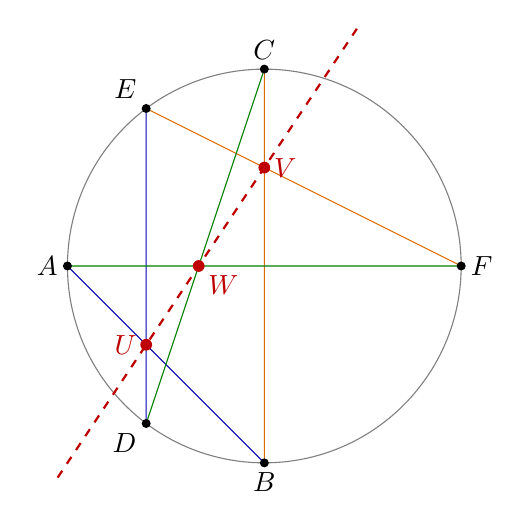
\begin{tikzpicture}[scale=2.5]
	\coordinate (A) at (-1,0);
	\coordinate (B) at (0,-1);
	\coordinate (C) at (0,1);
	\coordinate (D) at (-0.6,-0.8);
	\coordinate (E) at (-0.6,0.8);
	\coordinate (F) at (1,0);
	\draw[gray] (0,0) circle (1);
	\draw[blue!70!black] (A)--(B) (D)--(E);
	\draw[orange!85!black] (B)--(C) (E)--(F);
	\draw[green!50!black] (C)--(D) (F)--(A);
	\draw[red!75!black,thick,dashed] (-1.05,-1.075)--(0.47,1.205);
	\fill (A) circle (0.65pt) node[left]{\(A\)};
	\fill (B) circle (0.65pt) node[below]{\(B\)};
	\fill (C) circle (0.65pt) node[above]{\(C\)};
	\fill (D) circle (0.65pt) node[below left]{\(D\)};
	\fill (E) circle (0.65pt) node[above left]{\(E\)};
	\fill (F) circle (0.65pt) node[right]{\(F\)};
	\fill[red!75!black] (-0.6,-0.4) circle (0.85pt) node[left]{\(U\)};
	\fill[red!75!black] (0,0.5) circle (0.85pt) node[right]{\(V\)};
	\fill[red!75!black] (-0.333333,0) circle (0.85pt) node[below right]{\(W\)};
\end{tikzpicture}

	\caption[Pascal 的六点构形]{Pascal 的六点构形。三组同色的对边分别交于 \(U,V,W\)，红色虚线是它们的公共直线。六点的循环次序允许产生自交边。}
	\label{g1:fig:pascal}
\end{figure}

\cref{g1:fig:pascal}取单位圆上的
\[
	\begin{aligned}
		A&=(-1,0),&\qquad B&=(0,-1),\\
		C&=(0,1),& D&=(-3/5,-4/5),\\
		E&=(-3/5,4/5),& F&=(1,0).
	\end{aligned}
\]
这些点由\cref{g1:exm:circle-parametrization}的参数 \(\infty,-1,1,-2,2,0\) 给出。直线求交得到 \(U=(-3/5,-2/5)\)、\(V=(0,1/2)\)、\(W=(-1/3,0)\)，三点满足 \(y=3x/2+1/2\)。图中六边形虽有自交，关联关系仍然清楚。

\begin{example}[一个交点在无穷远处]\label{g1:exm:pascal-infinity}
	在定理的标准坐标中取 \(d=2\)、\(e=3\)、\(f=-2\)。则
	\[
		U=[-6:0:1],\qquad V=[-6:-6:0],\qquad W=[-8:-2:1].
	\]
	三个点都满足 \(X-Y+6Z=0\)。在仿射图 \(Z=1\) 中，\(BC\) 与 \(EF\) 是平行线，其交点 \(V\) 位于无穷远直线；因此仿射图像中的平行情形已经包含在同一个定理和证明里。
\end{example}

六点两两不同的条件使每条割线都有唯一含义。若相邻点重合，相应的边须改用切线，并要求剩下的交点仍有定义。

\subsection{Brianchon 定理与对偶推导}
\label{g1:subsec:0205:04}

\cref{g1:thm:pascal}涉及曲线上的点、两点连线、两线交点与共线。在对偶平面中，曲线点变成原平面中的切线，连线与交点互换，共线则变成共点。由此得到\term[Brianchondingli]{Brianchon 定理}[Brianchon's theorem]。\footnote{Charles-Julien Brianchon（1783--1864），法国数学家，研究射影几何与圆锥曲线。人物资料见University of St Andrews \href{https://mathshistory.st-andrews.ac.uk/Biographies/Brianchon/}{MacTutor 传记}。}下面逐一写出点、直线与关联关系的对偶对应。

\begin{table}[htbp]
	\centering
	\caption{Pascal 与 Brianchon 构形的对应}
	\label{g1:tab:pascal-brianchon}
	\begin{tabularx}{\textwidth}{@{}XXX@{}}
		\toprule
		Pascal 构形中的对象 & 对偶运算 & Brianchon 构形中的对象 \\
		\midrule
		圆锥曲线上的六点 & 点表示原平面的直线 & 六条不同的曲线切线 \\
		相邻两点的连线 & 张成与相交互换 & 相邻两条切线的交点 \\
		三组对边的交点共线 & 共线与共点互换 & 三条对角线通过公共点 \\
		\bottomrule
	\end{tabularx}
\end{table}

\cref{g1:tab:pascal-brianchon}列出的运算都来自零化子；证明还需要确认六条切线确实落在同一条对偶圆锥曲线上。

\begin{theorem}[Brianchon]\label{g1:thm:brianchon}
	设 \(K=\mathbb R\) 或 \(\mathbb C\)，\(\ell_1,\ldots,\ell_6\) 是 \(\mathbb P^2(K)\) 中一条非退化圆锥曲线的六条两两不同的切线。按循环次序置
	\[
		A=\ell_1\cap\ell_2,\quad B=\ell_2\cap\ell_3,\quad C=\ell_3\cap\ell_4,
		\quad D=\ell_4\cap\ell_5,\quad E=\ell_5\cap\ell_6,\quad F=\ell_6\cap\ell_1.
	\]
	则三条对角线 \(AD,BE,CF\) 共点。
\end{theorem}
\begin{proof}
	把每条 \(\ell_i\) 看作对偶平面中的点 \(L_i\)。由\cref{g1:thm:dual-quadric}，这六个不同的点位于一条非退化对偶圆锥曲线上。该曲线上没有三个不同点共线，这已在\cref{g1:thm:pascal}的证明中由参数二次式说明；由\cref{g1:prop:annihilator-duality}，原平面中的三条不同切线因而不共点。于是所列相邻交点存在，且 \(A\ne D\)、\(B\ne E\)、\(C\ne F\)，各对角线都有定义。

	在对偶平面对 \(L_1,\ldots,L_6\) 使用\cref{g1:thm:pascal}，得到
	\[
		U^*=L_1L_2\cap L_4L_5,\qquad
		V^*=L_2L_3\cap L_5L_6,\qquad
		W^*=L_3L_4\cap L_6L_1
	\]
	共线。直线 \(L_1L_2\) 是原平面中点 \(A\) 的对偶直线，\(L_4L_5\) 是原平面中点 \(D\) 的对偶直线；两条对偶直线的交点 \(U^*\) 因而对应原直线 \(AD\)。同理 \(V^*,W^*\) 分别对应 \(BE,CF\)。包含 \(U^*,V^*,W^*\) 的对偶直线对应原平面的一个点，关联反转保证该点同时属于 \(AD,BE,CF\)，即得结论。
\end{proof}

例如，在实平面取一条圆和一个外切六边形，三条对角线即使看上去没有明显对称性，仍然共点。定理不要求六条切线围成有界的凸区域，公共点也可能位于无穷远处；这些情形与前面允许割线平行的情形相对应。这说明对偶真正保留的是关联及其由线性方程表达的逻辑关系，长度、角度和“内外”都不是推导所需的数据。
